% Diese Zeile bitte -nicht- aendern.
\documentclass[course=erap]{aspdoc}

% Packages
\usepackage{amssymb}
\usepackage{xcolor}
\usepackage{pgfplots}
\usepackage[utf8]{inputenc}

% Definitions
\renewcommand{\figurename}{Abbildung}

%%%%%%%%%%%%%%%%%%%%%%%%%%%%%%%%%
%% TODO: Ersetzen Sie in den folgenden Zeilen die entsprechenden -Texte-
%% mit den richtigen Werten.
\newcommand{\theGroup}{215} % Beispiel: 42
\newcommand{\theNumber}{A500} % Beispiel: A123
\author{David Csida \and Georgios Merezas \and Fabian Degen}
\date{Sommersemester 2022} % Beispiel: Wintersemester 2019/20
%%%%%%%%%%%%%%%%%%%%%%%%%%%%%%%%%

% Diese Zeile bitte -nicht- aendern.
\title{Gruppe \theGroup{} -- Abgabe zu Aufgabe \theNumber}

\begin{document}
\maketitle

\section{Einleitung}
\subsection{Einführung}
Sei es beim Herstellen einer Verbindung mit einem Server oder das Chatten mit Freunden und Bekannten rund um
den Globus, nie genoss die Kryptographie mehr Relevanz als jetzt. Man möchte nicht, dass die Nachrichten,
die man an seine Geliebten versendet, von einer dritten Person mitgelesen werden können. Darum existieren
kryptographische Verfahren zur Verschlüsselung von Informationen. Eines dieser Ver\-schlüsselungs\-ver\-fahren ist
\emph{Salsa20/20}, welches es zu implementieren galt.

\subsection{Definitionen}
Im Folgenden bezeichne: 
\\ \hspace*{5mm} 1. $x \lll y$ die Linksrotation von $x$ um $y$ Bit. 
\\ \hspace*{5mm} 2. $\oplus$ den Binären XOR-Operator.

\subsection{Funktionsweise Salsa20/20}
Salsa20/20, im Folgenden auch Salsa20 genannt, ist eine Stromchiffre basierend auf einem sogenannten 
\emph{Add-Rotate-XOR-Schema} (kurz: ARX-Schema), ins Leben gerufen von David J. Bernstein.\\
Salsa20/20 verwendet eine 4$\times$4-Matrix bestehend aus vorzeichenlosen 32-bit \emph{Little-Endian-Ganzzahlen},
welche durch \emph{Add}, \emph{Rotate} und \emph{XOR} Operationen aus bestimmten Startwerten erzeugt wird.
Auf dieser generierten Matrix wird dann mit der zu ver\-schlü\-ssel\-nden Nachricht Byte für 
Byte eine XOR-Operation ausgeführt.

\subsubsection{Der Salsa20-Kern:}
Der Salsa20-Kern ist eine Funktion, welche einen 64-Byte Block generiert, auf dem, wie oben beschrieben, mit 
der zu verschlüsselnden Nachricht Byte für Byte eine XOR-Operation ausgeführt wird. Es werden bei jeder Operation 
zwei Werte der Matrix aufaddiert, links-rotiert und auf diesem Ergebnis mit einem Eintrag $a_{i,j}$ der Matrix eine XOR-Operation ausgeführt.
Der Matrixeintrag $a_{i,j}$ wird dann mit dem Ergebnis dieser XOR-Operation überschrieben.
Der 64-Byte-Block wird in 20 sogenannten Runden aus einem 256-Bit-Key, einer 64-Bit Nonce und einem 64-Bit 
Counter generiert. Die zwanzig Runden bestehen jeweils aus vier Viertelrunden. Die Viertelrunden unterscheiden sich 
durch die Anzahl der Rotationen, die für jede ARX-Operation ausgeführt werden und durch die Matrixeinträge, auf die 
diese Operationen angewandt werden. 
Zur Veranschaulichung, die erste Viertelrunde der Kernfunktion:
\[a_{2,1} = ((a_{1,1} + a_{4,1}) \lll 7) \oplus a_{2,1}\]
\[a_{3,2} = ((a_{2,2} + a_{1,2}) \lll 7) \oplus a_{3,2}\] 
\[a_{4,3} = ((a_{3,3} + a_{2,3}) \lll 7) \oplus a_{4,3}\] 
\[a_{1,4} = ((a_{4,4} + a_{3,4}) \lll 7) \oplus a_{1,4}\]
Am Ende jeder Runde wird die Matrix transponiert.
Den Startzustand $S$ für den generierten 64-Byte-Block bildet folgende 4$\times$4 Matrix, wobei $K_i$ den $i$-ten Teil
des Schlüssels bezeichnet. ($K_0$ steht also für die ersten 4 Bytes in Little-Endian-Reihenfolge des Schlüssels, dasselbe gilt analog für die
Nonce $N_i$ und den Counter $C_i$).
\[
    \begin{pmatrix}
    0\text{x}61707865 & K_0 & K_1 & K_2\\
    K_3 & 0\text{x}3320646\text{e} & N_0 & N_1\\
    C_0 & C_1 & 0\text{x}79622\text{d}32 & K_4\\
    K_5 & K_6 & K_7 & 0\text{x}6\text{b}206574
    \end{pmatrix}
\]
Die Konstanten auf der Diagonalen sind für jeden Key und jede Nonce dieselben.
Den zum Schluss ausgegebenen 64-Byte-Block erhält man duch das aufaddieren des 
Ergebnisses der 20 Runden auf den Startzustand $S$.

\subsection{Aufgabenstellung}

\subsubsection{Theoretischer Teil:}
Folgende theoretische Fragen waren zu beantworten:
\begin{itemize}
    \item Wie könnte man das im letzten Schritt einer jeden Salsa20-Kern Runde ineffiziente, stattfindende transponieren der Matrix optimieren?
    \item Was bedeuten die Werte an der Diagonalen des Startzustands?
    \item Erklären der Funktionsweise einer Stromchiffre anhand eines Beispiels. Warum kann man dieselbe Funktion zum Ver- und Entschlüsseln verwenden? Wie müssen die Parameter gewählt werden, damit dies funktioniert? Warum ist der Counter keine Eingabe des Verschlüsselungsalgorithmus?
\end{itemize}

\subsubsection{Praktischer Teil:}
Zu implementieren  war folgende Funktionalität:
\begin{itemize}
    \item Ein Rahmenprogramm welches I/O-Operationen unterstützt, mithilfe derer man eine ganze Datei in den Speicher einlesen und als Pointer an eine Unterfunktion übergeben kann. Selbiges soll auch zum Schreiben eines Speicherbereiches mit bekannter Länge in eine Datei möglich sein.
    \item \texttt{ \textcolor{blue}{void} salsa20\_core (\textcolor{blue} {uint32\_t} output[16], \textcolor{blue}{const uint32\_t} input[16])} \\
    Diese Funktion implementiert den oben beschriebenen Salsa20-Kern. input bezeichnet dabei den Startzustand des Kerns, output den finalen 64-Byte-Block. \\
    \item \texttt{ \textcolor{blue} {void} salsa20\_crypt (\textcolor{blue}{size\_t} mlen, \textcolor{blue} {const uint8\_t} msg[mlen], \textcolor{blue}{uint8\_t} cipher [mlen], \textcolor{blue}{uint32\_t} key[8], \textcolor{blue} {uint64\_t} iv) }\\
    Diese Funktion verschlüsselt eine Nachricht msg der Länge mlen mit einem gegebenen Schlüssel Key und einer Nonce (iv) und schreibt das Ergebnis in cipher.
\end{itemize}



\section{Lösungsansatz}
\subsection{Theoretischer Teil}
\subsubsection{Transponieren}

Das Transponieren der Matrix ist Teil des Salsa20-Kern Algorithmus, ist aber nicht sonderlich performant.
Um ihn weiter zu optimieren, kann man anstatt zwanzig Runden, die jeweils eine Transposition enthalten, zehn sogenannte Doppelrunden
ausführen, die jeweils aus einer sogenannten Spaltenrunde und einer Reihenrunde bestehen. Eine Spaltenrunde ist identisch zu einer
Runde wie oben definiert, während eine Reihenrunde die Indizes bei Matrixzugriffen so wählt, dass die Matrix behandelt wird
als wäre sie transponiert.
Wenn man zum Beispiel die erste ARX-Operation der Kernfunktion betrachtet:
\[
    a_{2,1} = ((a_{1,1} + a_{4,1}) \lll 7) \oplus a_{2,1} 
\]
Dann ist dies äquivalent zu folgender Operation, nachdem die Matrix A transponiert wurde:
\[
    a_{1,2} = ((a_{1,1} + a_{1,4}) \lll 7) \oplus a_{1,2}
\]

\subsubsection{Werte an der Diagonale}

Die Werte an der Diagonale haben eine wichtige Bedeutung für die Sicherheit des Salsa20/20 Algorithmus, insbesondere der Salsa20-Kern Funktion.
\vspace{1mm}
\\Betrachten wir im Folgenden eine Matrix $x$ und deren Transformation $tr(x)$:
\begin{gather*}
    x =
    \begin{pmatrix}
        A_0 & B_0 & C_0 & D_0 \\
        A_1 & B_1 & C_1 & D_1 \\
        A_2 & B_2 & C_2 & D_2 \\
        A_3 & B_3 & C_3 & D_3 \\
    \end{pmatrix}
    \quad \quad tr(x) =
    \begin{pmatrix}
        D_3 & D_2 & D_1 & D_0 \\
        C_3 & A_0 & B_0 & C_0 \\
        B_3 & A_1 & B_1 & C_1 \\
        A_3 & A_2 & B_2 & C_2
    \end{pmatrix}
\end{gather*}
Dann erhalten wir die folgende Eigenschaft:
\begin{gather*}
    Salsa20( tr(x) ) = tr( Salsa20(x) )
\end{gather*}
Diese Transformation der Matrix $x$ ist nicht nur invertierbar, sondern bleibt auch durch die Anwendung der Salsa-Funktion erhalten.\cite{salsa20security}
\vspace{1mm}
\\Nehmen wir nun die folgende Transformation der oben beschriebenen Matrix $x$:
\begin{gather*}
    R(x) =
    \begin{pmatrix}
        r(A_0) & r(B_0) & r(C_0) & r(D_0) \\
        r(A_1) & r(B_1) & r(C_1) & r(D_1) \\
        r(A_2) & r(B_2) & r(C_2) & r(D_2) \\
        r(A_3) & r(B_3) & r(C_3) & r(D_3) \\
    \end{pmatrix}
\end{gather*}
wobei $r(y)$ die Rechtsrotation des 4Byte großen $y$ um ein Bit darstellt.
\vspace{1mm}
\\Dann erhalten wir eine äquivalente Eigenschaft wie schon mit $tr(x)$:
\begin{gather*}
    Salsa20(R(x)) = R(Salsa20(x))
\end{gather*}
Diese Transformation ist ebenfalls invertierbar und bleibt auch, in den meisten Fällen, nach Anwendung der Funktion Salsa20 erhalten.\cite{salsa20security}
\vspace{1mm}
\\Da diese Matrixverschiebungen und Rechtsrotationen \textbf{beide} sowohl invertierbar sind als auch mit der Anwendung von der Salsa20-Kern Funktion erhalten bleiben,
kann man eine Vielzahl von \textbf{beiden} auf die ursprüngliche Matrix anwenden und am Ende der Salsa20-Kern Funktion, unabhängig von der Reihenfolge des Anwendens, immer noch dasselbe Ergebnis erhalten.
\vspace{1mm}
\\Beim verwenden der Salsa20-Kern Funktion mit beliebigen Matrizen stellen diese Eigenschaften ein großes Sicherheitsrisikio dar.
Bei kryptographischen Verfahren ist das Ziel normalerweise, die Struktur so zu zerstören, dass ein Angriff sie nicht wiederherstellen kann.
Die Verschiebungen und Bitrotationen werden von der Funktion jedoch in keiner Weise beeinflusst.
\vspace{1mm}
\\An dieser Stelle kommen die Konstanten auf der Diagonale ins Spiel:
\vspace{2mm}
\\Durch die Einführung dieser Konstanten wird sichergestellt, dass keine Anzahl an Verschiebungen oder Rotationen die ursprüngliche Diagonale wiederherstellen kann,
außer im trivialen Fall von 0 Verschiebungen und Rotationen. Das bedeutet, dass keine zwei verschiedenen Schlüssel- oder Nonce-Eingaben
jemals die gleiche Matrix haben werden, egal wie viele Transformationen angewendet werden.\cite{salsa20security}
\vspace{1mm}
\\Natürlich sind nicht alle Werte geeignet, denn es gibt einige Beispiele für Konstanten,
wo die Diagonale nach einer bestimmten Anzahl von Verschiebungen/Rotationen mit der Originalen übereinstimmt.
\vspace{1mm}
\\Außerdem stellt der Ersteller des Algorithmus fest\cite{ResponseOnTheSalsa20Core}, dass die Konstanten das Kollisionsproblem beseitigen,
auf das in einer anderen Arbeit\cite{onTheSalsa20Core} hingewiesen wurde.\\
Das Kollisionsproblem besagt, dass:
\begin{gather*} Salsa20(x) = Salsa20(x + \Delta) \text{  mit z.B.  } \Delta=(0x80000000,0x80000000,...) \end{gather*}
Ein solches $x+\Delta$ ist aber keine gültige Eingabe für eine Salsa20-Kern Funktion (sofern $x$ eine gültige Eingabe ist) und wird daher in der Praxis nie vorkommen.
Das Gleiche gilt für andere Beispiele von Kollisionen, die in dieser Arbeit auftauchen.


\subsubsection{Funktionsweise einer Stromchiffre} \label{streamcipher}
Eine Stromchiffre ist ein symmetrischer kryptographischer Algorithmus, der für Ver- und Entschlüsselung von Daten verwendet wird.
Dieser Algorithmus nimmt einen Klartext und ein Schlüsselstrom entgegen und führt eine bitweise XOR-Operation aus und gibt am Ende
einen Geheimtext zurück.
Man kann durch Benutzung desselben Schlüsselstroms wieder den Klartext erhalten, indem man dem Algorithmus den Geheimtext übergibt.
% TODO: Beispiel von Klartext, Strom und Cipher
Aufgrund der Symmetrie der XOR-Operation gilt folgendes:
\begin{table}[!h]
    \begin{tabular}{|c|c|c|}
        \hline
        Klartext & Schlüsselstrom & Geheimtext \\
        \hline
        0        & 0              & 0          \\
        0        & 1              & 1          \\
        1        & 0              & 1          \\
        1        & 1              & 0          \\
        \hline
    \end{tabular}
    \begin{tabular}{|c|c|c|}
        \hline
        Geheimtext & Schlüsselstrom & Klartext \\
        \hline
        0          & 0              & 0        \\
        1          & 1              & 0        \\
        1          & 0              & 1        \\
        0          & 1              & 1        \\
        \hline
    \end{tabular}
\end{table}
\\
Wie man sehen kann, führt der Geheimtext als Eingabe unter Verwendung desselben Schlüsselstroms wieder zum Klartext.
\vspace{3mm}
\\
Damit man also für einen durch Salsa20/20 erstellten Geheimtext den dazugehörigen Klartext zurückerhält,
muss man denselben Schlüssel sowie denselben Initalisierungsvektor, mit dem Geheimtext als zu verschlüsselnde Nachricht, übergeben.
\\
Der Counter ist keine Eingabe des Salsa20/20 Verschlüsselungsverfahren, sondern dient dazu den generierten 64-Byte-Block sicherer gegen Angriffe zu machen. 
Alle 64 verschlüsselte Bytes, wird der Counter um 1 inkrementiert und der Kern neu berechnet. Das macht es schwerer, den Kern vorherzusagen und bietet somit mehr Sicherheit für das Verschlüsselungsverfahren und schützt den Geheimtext gegen Angriffe.


\subsection{Praktischer Teil}
\subsubsection{Das Rahmenprogramm}
Im Rahmenprogramm finden die von der Aufgabenstellung erforderlichen I/O-Operationen, sowie das Parsen von Programmargumenten statt.
Für das Einlesen des Eingabe Files wurden die von C bereitgestellten Funktionen zur File I/O verwendet. Das Einlesen der Programmargumente stellte nur für den 256bit Schlüssel
ein Problem dar, da für so große Eingabe Zahlen keine von C bereitgestellte sichere Funktion (wie z.B. strtoull für unsigned long long Zahlen) existiert.
Um diesen Problem nachzugehen wurde folgender Ansatz gewählt:
Der Key lässt sich entweder als Hexadezimalzahl eingeben, indem man das Präfix 0x anfügt, oder alternativ ohne Präfix, wo jeder Eingabecharacter als sein Zugehöriger numerischer Wert
nach ASCII-Codierung interpretiert wird.
\\Die Eingabe 
\begin{center}
  \texttt{./salsa -k 0x48656C6C6F576F726C64  some\_path}
\end{center} 
wäre also äquivalent zur Eingabe
\begin{center}
   \texttt{./salsa -k ``Hello World'' some\_path}
\end{center}
Diese Designentscheidung wurde getroffen, da z.B. eine Eingabe als dezimale Zahlen zu erlauben sehr aufwändig gewesen wäre, denn zusätzlich zur maximalen Länge wäre auf over- bzw. underflows und diverse andere Probleme wie zum
Beispiel führende Nullen oder unerlaubte Zeichen zu prüfen gewesen. Hexadezimalzahlen lassen sich jedoch sehr leicht konvertieren, genauso wie Strings interpretiert als ihre zugehörigen numerischen ASCII-Code Werte.
\\Das schreiben ins Outputfile findet statt, als die respektiven Bytes der cipher aneinandergehängt ausgegeben in hexadezimaler Form, mit einer neuen Zeile alle 76 Zeichen für bessere Lesbarkeit.
Für den Fall, dass jedes Byte der Cypher einem darstellbaren ASCII Character enstpricht, so findet die Ausgabe in ASCII Charactern statt. Diese Designentscheidung wurde getroffen, 
da eine Ausgabe mithilfe von fwrite unbrauchbar ist, weil frwite nur die Binärdaten in das Outputfile schreibt, wohingegen eine Ausgabe in hexadezimaler Form tatsächlich lesbar ist.
Das eine vollständig in ASCII darstellbare cipher auch in ASCII ausgegeben wird, dient der Entschlüsselung von bereits verschlüsselten Files.
Das führt zwar zu einer längeren Laufzeit, da erst überprüft werden muss ob die cipher als ASCII Character dargstellt werden kann ist aber unverzichtbar um bei der Entschlüsselung Klartexte und keine Hexadezimalzahlen zu erhalten.
Der Einfachheit halber werden jedoch nur ASCII Characters im Wertebereich von [32;126] akzeptiert, das heißt insbesondere sind Umlaute nicht unterstüzt. Nicht unterstützt bedeutet in diesem Fall dass eine Entschlüsselung von bereits 
verschlüsselten Klartexten, die einen Wert außerhalb des Wertebereichs enthalten, nicht den ursprünglichen Klartext zurückliefert.
\\Beispiel: 
\\Bezeichne im folgenden some\_path den Pfad eines Text-Files mit folgendem Inhalt:
\begin{center}
    Hallo ich soll verschluesselt werden.
\end{center}
Dann liefer folgender Aufruf
\begin{center}
    ./salsa some\_path
\end{center}
als Ergebnis im neu erstellen File result.txt
\begin{center}
    ffaf8cc85945bbe69fb07860173e0f855ebe070b80c82b91922bcab1f0d85208fde3c49610
\end{center}
Sei path\_of\_result der Pfad des gerade erstellten Files result.txt. Dann liefert der Aufruf
\begin{center}
   ./salsa path\_of\_result
\end{center}
das Egebnis (wieder in result.txt, da kein Pfad vom Benutzer angegeben wurde)
\begin{center}
    Hallo ich soll verschluesselt werden.
\end{center}

\subsubsection{salsa20\_core}
In der Funktion salsa20\_core wird das Verhalten der in Abschnitt 1.2.1 beschriebenen Salsa20-Kern Funktion exakt nachempfunden. Für die Implementierung V1 wurden jedoch kleine Änderungen vorgenommen.
Als Ansatz zur Optimierung wurden hier die 20 Runden auf nur 10 Runden reduziert, in denen man jedoch die doppelte Arbeit verrichtet. Es ist also eine Art loop unrolling mit zusätzlichem einsparen des 
transponierens der Matrix. Anstatt zu transponieren werden also einfach nochmals alle ARX-Operationen durchgeführt, jedoch werden die Indizes der Matrix so behandelt, als würde man bereits auf
der transponierten Matrix arbeiten. Somit spart man sich in jedem Schritt das transponieren der Matrix ein, und führt zusätzlich pro Schleifendruchlauf gleich 2 Arbeitsschritte durch. Implementierung V2
arbeitet auf die gleiche Weise wie Implementierung V1, nur das hier zusätzlich, unter Zuhilfenahme von SIMD Instruktionen, eine Viertelrunde vektorisiert ausgeführt wird. Eine Viertelrunde bestand zuvor 
aus vier nacheinander ausgeführten ARX-Operationen, die jetzt gleichzeitig vollzogen werden. Auf eine Vektorisierung der Addierung der Ergebnismatrix aus den 10 durchgeführten Runden auf den Startzustand wurde verzichtet,
da der Overhead der Lade- und Schreiboperationen den Speedup bei der Addition zunichte macht.
\\Als Standardwerte für Key und Nonce wurde sich, jeweils für den respektiven Wertebereich, für große Primzahlen enschieden. Ein fester Wert für diese beiden Parameter stellt in Realität ein großes Sicherheitsrisiko dar, 
da ein Angreifer nur diese beiden Werte benötigen würde, um jedes mit diesen Werten verschlüsselte File wieder zu entschlüsseln. In dieser Implementierung wurden jedoch feste Standardwerte verwendet, einerseits aus Gründen
der Einfachheit, andererseits um besser testen zu können. Man könnte in einer reellen Anwendung zum Beispiel anhand eines vom User eingebenen Passworts, 
eindeutige Werte für Key und Nonce berechnen, um das File zu verschlüsseln. Wenn der User nun sein File entschlüsseln möchte, kann er sein Passwort eingeben und es werden dieselben Werte für Key und Nonce berechnet, anhand derer
das File wieder entschlüsselt werden kann.

\subsubsection{salsa20\_crypt} \label{crypt}
Die salsa20\_crypt Funktion wird in allen Implementierungen erstmal der Startzustand der Matrix initalisiert. Für die Little-Endian-Reihenfolge des Keys, der Nonce und des Counters werden built\_in Funktionen verwendet.
Anschließend wird mithilfe eines Pointercasts des output Pointers (\texttt{\textcolor{blue}{uint32\_t}}) zu einem \texttt{\textcolor{blue}{uint8\_t}} Pointer die XOR-Operationen durchgeführt. Dieser Pointercast stellt kein Undefined Behaviour dar, 
da \texttt{\textcolor{blue}{uint8\_t}} keine strengeren alignment Anforderungen hat als \texttt{\textcolor{blue}{uint32\_t}}. Des weiteren liefert der Pointercast die Bytes der output Matrix für die XOR-Operation, genau wie vorgesehen, in Little-Endian-Reihenfolge.
Anschließend werden nun die XOR-Operationen auf der message mit der output Matrix ausgeführt und in cipher gespeichert. Alle 64 XOR-Operationen wird der Counter inkrementiert und der Kern neu berechnet. Für V1 wird nur für die letzten $\leq 64$ Bytes mit dem Pointercast gearbeitet.
Zuvor werden die XOR-Operationen mit der Berechnung des korrekten Index innerhalb der Matrix, der cipher und der message durchgeführt. Das reicht jedoch bereits für einen Signifikanten Speedup, dazu mehr in Abschnitt 4.
Die Implementierung V2 basiert nahezu vollständig auf der Implementierung von V1, nur mit zusätzlicher Vektorisierung der XOR-Operation mithilfe von SIMD Operationen.


\section{Korrektheit}
Im Folgenden wird auf die Korrektheit der Hauptimplementierung eingegangen.
Es wird \textbf{nicht} auf die Genauigkeit des Programms eingegangen, da es bei Ver\-schlüsse\-lungsverfahren
nur richtig oder falsch und eben kein ``ungenau'' gibt.
\\
Die Korrektheit unserer Implementationen des Salsa20/20 kyptographisches Verfahrens haengt von der Korrektheit der Kryptfunktion und der Kernfunktion, sowie vom Einlesen des Schluessels an. (Das Einlesen vom Nonce nutzt Funktionen der standard Bibliothek, von denen wir annehmen können, dass sie korrekt sind).

\subsection{Einlesen vom Schluessel}
Beim Einlesen es ist unerheblich, ob wir ein hex Nummer oder ein String eingeben, da sie auf die gleiche Weise interpretiert werden, auch wenn sie einen etwas anderen Algorithmus erfordern, um sie in ein Array von uint32\_t zu parsen. [reference to key]
Um dann die Korrektheit des Parsings der Eingabe zu überprüfen, müssen wir nur einige repräsentative Unit-Tests schreiben, die als Eingabe einen String haben, wie man ihn von der Eingabe als optarg erhalten würde, und vergleichen die Ausgabe der void convert\_string\_to\_uint32\_t\_array(const char *string, uint32\_t key[8]) mit einem erwarteten Array.
Man kann dazu auch einige Testfaelle schreiben, die die Ergebnisse zwischen gleichwertige Eingabe jeweils in hex und string vergleichen.


\subsection{Die Kryptfunktion}
Die Funktionsweise der Kryptfunktion nutzt XOR Operationen um die message mit der Ausgabe von der Kernfunktion zu Verschluesseln [reference to crypt beschreibung]

Wie bereits im theoretischen (Abschnitt \ref{streamcipher}) und praktischen (Abschnitt \ref{crypt}) Teilen des Loesungsansatzes gezeigt,
 die XOR Operation ist zum Ver- und Entschluesselung benutzt. 
 Um also die Korrektheit der Kryptfunktion zu testen, müssen wir nur einige repräsentative manuelle
  und eine Menge automatisierter Zufallstests schreiben, die die Kryptfunktion zweimal aufrufen.
  Beim ersten Aufruf ist dann die Eingabe eine message-Array, die Ausgabe ist eine Chiffre, 
  beim zweiten Aufruf ist die Eingabe diese Chiffre und die Ausgabe ein anderes Array. 
  Am Ende vergleichen wir das ursprüngliche message-Array mit dem Array, das nach dem zweiten 
  Funktionsaufruf ausgegeben wird.


\subsection{Die Kernfunktion}
Die Spezifikationen der Kernfunktion werden in dieser Arbeit beschrieben \cite{salsa20specification}

Um unsere Implementierung dieser Funktion zu testen, wurde beschlossen, die vom Autor selbst in C geschriebene Referenzimplementierung zu verwenden \cite{salsa20}
Der Aufruf dieser Referenzimplementierung für eine Menge von Eingaben und auch eine der Versionen unserer Implementierung mit denselben Eingaben sollte dann dieselbe Chiffre ergeben, wenn die Version tatsächlich korrekt implementiert wurde. 
Auch hier kann man einige repräsentative manuelle Tests und eine Menge von automatisierten Zufallstests schreiben, um zu pruefen, ob das eigentlich stimmt. 

Es können auch einige manuelle Tests geschrieben werden, die die Kernfunktion direkt aufrufen und dabei die Eingabe und die erwartete Ausgabe aus Abschnitt 8 "Die Salsa20-Hash-Funktion" der Spezifikation verwenden \cite{salsa20specification}.



Die obengenannten Tests können mit der Option -t X aufgerufen werden, wobei X für die Anzahl der automatisierten Tests steht, die durchgeführt werden. Die manuellen Tests werden in ihrer Gesamtheit durchgeführt, unabhängig davon, was X ist. Um die verschiedene Implementationen zu testen, man kann das Programm mit -V X ausfuehren, wobei X fuer die jeweilige Implementation (0,1 oder 2) steht.


\section{Performanzanalyse}
\subsection{Vergleich der Implementierungen}
Es wurden pro GCC-Optimierungsstufe und Implementierungsversion 25 
Iterationen des Verfahrens auf einer 100MB großen Datei ausgeführt. Die Datei
wurde durch den Befehl \texttt{base64 /dev/urandom | head -c 100000000 > 100mb.txt}
erzeugt.
Die Laufzeiten wurden vom Rahmenprogramm selbst durch setzen des -B Flags
gemessen. Getestet wurde auf einem Notebook mit einem AMD Ryzen 7 5800H, 
4.4GHz, 16 GiB Arbeitsspeicher, Fedora 36, 64 Bit, Linux Kernel 5.18.11.
Kompiliert wurde mit GCC 12.1.1 mit den Optionen \texttt{O0}, \texttt{O2} und \texttt{O3}.

\begin{center}
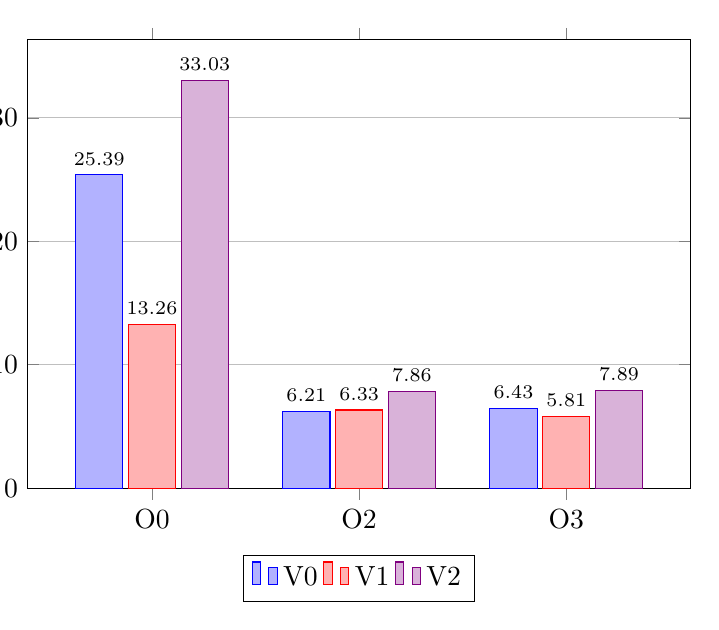
\begin{tikzpicture}[trim axis left, trim axis right]
    \begin{axis}[
            symbolic x coords={O0, O2, O3},
            xtick = {O0, O2, O3},
            legend style={at={(0.5,-0.15)},
                    anchor=north,legend columns=-1},
            ybar,
            ymin=0,
            ymajorgrids=true,
            ylabel=Sekunden pro Iteration,
            bar width=6mm,
            width=100mm,
            height=\axisdefaultheight,
            enlarge x limits=0.3,
            nodes near coords,
            every node near coord/.append style={font = {\fontsize{7 pt}{12 pt}\selectfont},color=black},
        ]
        \addplot[blue,fill=blue!30]
        coordinates {(O0,25.39) (O2,6.21)
                (O3,6.43) };

        \addplot[red,fill=red!30]
        coordinates {(O0,13.26) (O2,6.33)
                (O3,5.81) };

        \addplot [violet,fill=violet!30]
        coordinates {(O0,33.03) (O2,7.86)
                (O3,7.89) };
        \legend{V0,V1,V2}
    \end{axis}
\end{tikzpicture}
\captionof{figure}{Laufzeiten der Implementierungen}
\label{diagram1}
\end{center}
Wie in Abbildung \ref{diagram1} zu sehen ist, gibt es bei Kompilierung mit \texttt{O0} starke
Unterschiede in den Laufzeiten der drei Implementierungen. V1 ist deutlich schneller als V0 
und V2 wiederum deutlich langsamer. Durch Kompilierung mit \texttt{O2} beziehungsweise \texttt{O3}
konnte die Performanz aller drei Implementierungen merkbar verbessert werden und der Laufzeitnachteil
von V0 minimiert werden.

\subsection{Analyse der Performanzmessungen}
Durch Analyse der drei Implementierung mit dem Tool \emph{perf} - unter 
den gleichen Testbedingungen als zuvor, mit der Änderung, dass nur mit \texttt{O0} kompiliert wurde 
- zeigt sich, warum V1 etwas schneller als V0 ist und warum V2 langsamer ist.
Um eine übersichtliche Dartstellung zu ermöglichen, wurden die Funktionen \texttt{salsa20\_core},
\texttt{rowRound} und \texttt{columRound} zu \texttt{salsa20\_core} zusammengefasst. Weiters wird angemerkt, dass
Funktionssuffixe wie \texttt{\_v1} weggelassen werden.

\begin{center}
    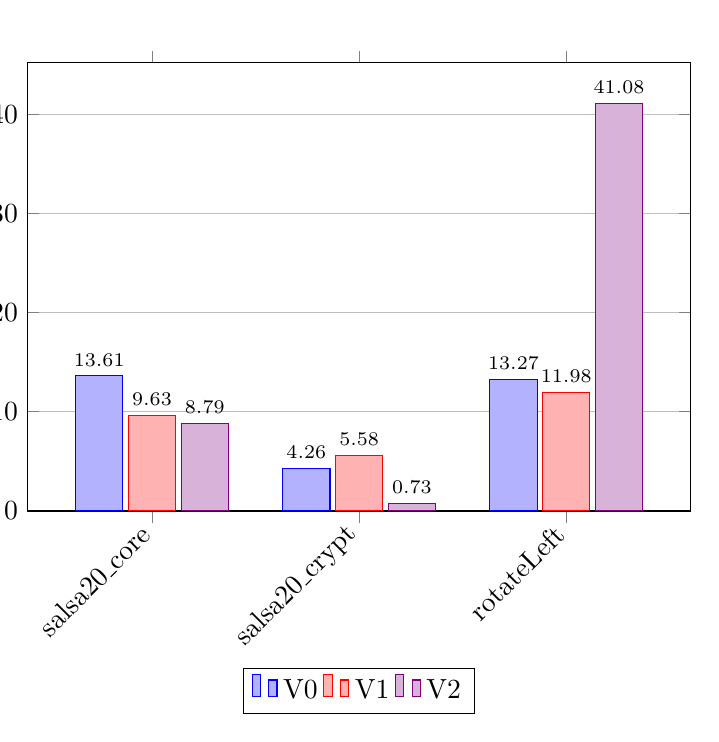
\begin{tikzpicture}[trim axis left, trim axis right]
        \begin{axis}[
                symbolic x coords={salsa20\_core, salsa20\_crypt, rotateLeft},
                xtick = {salsa20\_core, salsa20\_crypt, rotateLeft},
                x tick label style={rotate=45, anchor=east, align=center},
                legend style={at={(0.5,-0.35)},
                        anchor=north,legend columns=-1},
                ybar,
                ymin=0,
                ymajorgrids=true,
                ylabel=Anteil an der Ausführungszeit in Prozent,
                bar width=6mm,
                width=100mm,
                height=\axisdefaultheight,
                enlarge x limits=0.3,
                nodes near coords,
                every node near coord/.append style={font = {\fontsize{7 pt}{12 pt}\selectfont},color=black},
            ]
            \addplot[blue,fill=blue!30]
            coordinates {(salsa20\_core,13.61)
            (rotateLeft,13.27) (salsa20\_crypt,4.26)};
    
            \addplot[red,fill=red!30]
            coordinates {(salsa20\_core,9.63)
                    (rotateLeft,11.98) (salsa20\_crypt,5.58)};
    
            \addplot[violet,fill=violet!30]
            coordinates {(salsa20\_core,8.79)
                    (rotateLeft,41.08) (salsa20\_crypt,0.73)};
    
            \legend{V0,V1,V2}
        \end{axis}
    \end{tikzpicture}
    \captionof{figure}{Relative Laufzeiten der Implementierungen}
\label{diagram2}
\end{center}
Aus den erhobenen Daten geht hervor, dass der Hauptgrund für den Performanzvorteil von 
V1 gegenüber V0 (bei Kompilierung mit O0) bei \texttt{salsa20\_core} liegt, vermutlich da hier auf das 
Transponieren der Matrix verzichtet wird.
Die Unterschiede bei \texttt{salsa20\_crypt} und \texttt{rotateLeft} sind deutlich geringer und vermutlich dadurch
entstanden, da der Anteil von \texttt{salsa20\_core} in V1 deutlich gesunken ist. V0 und V1 verwenden beide
dieselbe Implementierung von \texttt{rotateLeft} und \texttt{salsa20\_crypt} unterscheidet sich hier auch nur minimal
wie in Abschnitt \ref{crypt} genauer beschrieben. Während V1 merkbar schneller als V0 ist, ist V2 in Abbildung 
\ref{diagram1} signifikant langsamer als die beiden anderen Implementierungen. Dies liegt hauptsächlich an \texttt{rotateLeft}, 
das für V2 mit SIMD-Instruktionen umgesetzt wurde. Durch das Verwenden des \emph{annotate}-Features von 
\emph{perf}, erkennt man, dass die meiste Zeit der Laufzeit in rotateLeft in V2 für \texttt{mov}-Operationen in 
\emph{xmm}-Register verwendet wird. Anzumerken ist, dass die XOR-Operationen, die in den beiden anderen Implementierungen
in \texttt{salsa20\_core} stattfinden, in V2 stattdessen in \texttt{rotateLeft} geschehen, was sich aber nur gering 
auf die Messung auswirkt, da laut \emph{perf} die Instruktion \texttt{pxor} nur zu einem geringen 
Prozentsatz von < 0.1\% zur Laufzeit beiträgt.
Dadurch, dass \texttt{rotateLeft} in V2 einen beträchtlichen Teil der Laufzeit in Anspruch nimmt,
haben \texttt{salsa20\_core} und \texttt{salsa20\_crypt} wahrscheinlich einen geringeren Anteil an der Laufzeit. Es kann 
also nicht festgestellt werden, ob die beiden Funktionen optimiert werden konnten.


\section{Zusammenfassung und Ausblick}
Ziel dieses Gruppenprojekts war es, das Salsa20-Verschlüsselungsverfahren in C umzusetzen und zu optimieren.

\subsection{Ansatz}
Der gewählte Ansatz war zuerst das Rahmenprogramm und die Hauptimplementierung V0 umzusetzen 
und zwei alternative Implementierungen anzufertigen. Die Hauptimplementierung sollte genau wie 
in der Aufgabenstellung beschrieben umgesetzt werden.
Die erste Alternativimplementierung V1 sollte nur die Transposition der $4\times 4$-Matrix aus 
dem Algorithmus entfernen und durch Verwendung transponierter Indizes ersetzt werden. Die zweite Alternative V2
sollte denselben Algorithmus wie die erste verwenden, aber zusätzlich wo möglich \emph{SIMD}-Instruktionen verwenden.

\subsection{Ergebnisse}
V0 konnte erfolgreich umgesetzt werden und V1 konnte 
diese erfolgreich verbessern. Durch weitere Optimierungen von \emph{GCC} wurde die V0 aber
genauso performant.
Eine weitere Performanzsteigerung durch den Einsatz von SIMD-Instruktionen konnte jedoch nicht erreicht werden
und es wurde sogar eine starke Performanzverminderung von V2 gegenüber der beiden anderen Implementierungen erreicht.

\subsection{Verbesserungspotenzial}
Durch klügeres und vor allem weniger häufiges Bewegen von Werten in und aus \emph{xmm}-Register heraus
in V2 hätte vermutlich ein Speedup erreicht werden können, sodass V2 die performanteste Implementierung
geworden wäre.
Weiters könnte der I/O-Teil des Rahmenprogramms dahingehend verbessert werden, dass auch Dezimal- und
Oktalzahlen als Eingabe entgegengenommen werden können. Allgemein hätte das Rahmenprogramm auch mit einem 
TUI umgesetzt werden können, sodass Optionen graphisch ausgewählt werden können.



% TODO: Fuegen Sie Ihre Quellen der Datei Ausarbeitung.bib hinzu
% Referenzieren Sie diese dann mit \cite{}.
% Beispiel: CR2 ist ein Register der x86-Architektur~\cite{intel2017man}.
\bibliographystyle{plain}
\bibliography{Ausarbeitung}{}

\end{document}